% Phase 2 -- written by Abdullah, numbers updated after the top-up re-run (19 Oct)
% NOTE: every number below comes from the terminal output of clean_data.py and
% preprocess.py, from data/cleaning_report.csv, or from the raw image counts.
% If the dataset changes again, re-run the scripts and update every number here.
% TODO markers (comments) mark sentences that describe the charts and must be
% re-checked against the figures generated by the final run.
\section{Phase 2: Data Acquisition and Preprocessing}

\subsection{Collection}
Raw images were collected from two sources, giving 6,193 images across the 14 dishes before any cleaning. Kaggle contributes 1,154 of them and Bing scraping the remaining 5,039.

\paragraph{Bing image scraping.} The script \texttt{collect\_images.py} downloads images from Bing using the \texttt{icrawler} package, with five query variants per dish (for example the plain dish name, ``Pakistani'', ``homemade'' and ``restaurant plate''). Every downloaded URL is logged in \texttt{raw\_metadata.csv}, so each image can be traced back to where it came from.

\paragraph{Kaggle dataset.} The script \texttt{import\_dataset.py} imports four classes from the Kaggle ``Indian Food Classification'' dataset (Pushkar Jain, Kaggle user \texttt{l33tc0d3r}) and maps them onto our dishes: \texttt{samosa} $\rightarrow$ samosa (262 images), \texttt{pakode} $\rightarrow$ pakora (278), \texttt{dal\_makhani} $\rightarrow$ daal (321) and \texttt{kaathi\_rolls} $\rightarrow$ paratha\_roll (293). The remaining ten dishes come only from Bing.

\paragraph{Top-up scraping.} After the first cleaning run, three dishes were below or close to our target of 150 images: chicken\_karahi (128 images), aloo\_gosht (167) and halwa\_puri (171). We re-ran \texttt{collect\_images.py} for these three dishes only, using its \texttt{--dishes} and \texttt{--set extra} options, which apply eight different search phrasings (for example ``recipe'', ``dhaba style'', ``Lahore'' and ``home cooked'') with up to 60 results each. This added 1,180 raw images (chicken\_karahi 410, aloo\_gosht 382, halwa\_puri 388). Many of the new downloads duplicated images we already had, so cleaning removed a larger share from these three dishes (see Table~\ref{tab:perdish}). The cleaning and preprocessing scripts were then re-run on the combined collection, and all numbers in this report refer to that final run.

\begin{table}[H]
  \centering
  \begin{tabular}{|l|r|l|}
    \hline
    \textbf{Dish} & \textbf{Raw images} & \textbf{Source} \\
    \hline
    halwa\_puri     & 702 & Bing \\
    chicken\_karahi & 639 & Bing \\
    daal            & 636 & Bing + Kaggle (dal makhani, 321) \\
    aloo\_gosht     & 624 & Bing \\
    paratha\_roll   & 566 & Bing + Kaggle (kathi rolls, 293) \\
    samosa          & 556 & Bing + Kaggle (samosa, 262) \\
    pakora          & 525 & Bing + Kaggle (pakode, 278) \\
    seekh\_kebab    & 317 & Bing \\
    chicken\_biryani & 296 & Bing \\
    nihari          & 291 & Bing \\
    chicken\_tikka  & 289 & Bing \\
    pulao           & 261 & Bing \\
    haleem          & 254 & Bing \\
    palak\_paneer   & 237 & Bing \\
    \hline
    \textbf{Total}  & \textbf{6,193} & \\
    \hline
  \end{tabular}
  \caption{Raw images per dish and their source, before cleaning (including the top-up scraping).}
\end{table}

\subsection{Cleaning Implementation}
Cleaning is done by \texttt{clean\_data.py}, which never deletes the raw files: the images that pass are copied into a separate \texttt{data/clean} folder, together with \texttt{clean\_metadata.csv} and \texttt{cleaning\_report.csv}. The script applies the following checks:
\begin{itemize}
  \item \textbf{Missing labels and duplicate metadata rows:} rows with no dish label, or repeated rows, are dropped.
  \item \textbf{Missing or corrupt files:} images that are not on disk or cannot be opened are dropped.
  \item \textbf{Tiny images:} images whose shorter side is below 150 pixels are dropped.
  \item \textbf{Extreme aspect ratio:} images with an aspect ratio above 3 are dropped.
  \item \textbf{Blur:} images whose Laplacian variance is below 40 are dropped as blurry.
  \item \textbf{Exact duplicates:} images with an identical MD5 hash are dropped.
  \item \textbf{Near duplicates:} images whose perceptual hash distance to an earlier image is at most 4 are dropped.
\end{itemize}
The script also records the width, height, brightness and blur score of every kept image, which are used for the exploratory analysis. Of the 6,193 raw images, 1,926 (31.1\%) were removed and 4,267 (68.9\%) were kept. Table~\ref{tab:cleaning} shows what each step removed, as reported in \texttt{cleaning\_report.csv}; the report does not list separate counts for the missing-file, corrupt-file and tiny-image checks.

\begin{table}[H]
  \centering
  \begin{tabular}{|l|r|}
    \hline
    \textbf{Cleaning step} & \textbf{Images removed} \\
    \hline
    Missing label                          & 0 \\
    Duplicate metadata rows                & 0 \\
    Exact duplicates (MD5)                 & 1,390 \\
    Blurry (Laplacian variance $<$ 40)     & 253 \\
    Near duplicates (perceptual hash $\leq$ 4) & 278 \\
    Extreme aspect ratio ($>$ 3)           & 5 \\
    \hline
    \textbf{Total removed}                 & \textbf{1,926} \\
    \textbf{Images kept}                   & \textbf{4,267} \\
    \hline
  \end{tabular}
  \caption{Images removed by each cleaning step (from \texttt{cleaning\_report.csv}).}
  \label{tab:cleaning}
\end{table}

Table~\ref{tab:perdish} gives the effect of cleaning on each dish. We also checked a random sample of 24 cleaned images from each of the three top-up dishes by eye. The dish was almost always correct and the images were sharp, but text and watermarks were common: about 12 of 24 sampled aloo\_gosht images and about 12 of 24 halwa\_puri images contained a text banner, a video-thumbnail graphic or a stock-photo watermark, against about 5 of 24 for chicken\_karahi. This is a small sample, so these rates are only rough (see the limitations below).

\begin{table}[H]
  \centering
  \begin{tabular}{|l|r|r|}
    \hline
    \textbf{Dish} & \textbf{Raw} & \textbf{Kept after cleaning} \\
    \hline
    samosa          & 556 & 498 \\
    pakora          & 525 & 482 \\
    daal            & 636 & 461 \\
    paratha\_roll   & 566 & 422 \\
    chicken\_karahi & 639 & 295 \\
    aloo\_gosht     & 624 & 286 \\
    halwa\_puri     & 702 & 263 \\
    chicken\_biryani & 296 & 248 \\
    seekh\_kebab    & 317 & 241 \\
    nihari          & 291 & 236 \\
    haleem          & 254 & 227 \\
    chicken\_tikka  & 289 & 224 \\
    pulao           & 261 & 197 \\
    palak\_paneer   & 237 & 187 \\
    \hline
    \textbf{Total}  & \textbf{6,193} & \textbf{4,267} \\
    \hline
  \end{tabular}
  \caption{Images per dish before and after cleaning.}
  \label{tab:perdish}
\end{table}

\subsection{Feature Strategy}
The script \texttt{preprocess.py} prepares the cleaned images for model training in the following way.

\paragraph{Label encoding.} The 14 dish names are sorted alphabetically and mapped to integer ids: aloo\_gosht = 0, chicken\_biryani = 1, chicken\_karahi = 2, chicken\_tikka = 3, daal = 4, haleem = 5, halwa\_puri = 6, nihari = 7, pakora = 8, palak\_paneer = 9, paratha\_roll = 10, pulao = 11, samosa = 12 and seekh\_kebab = 13. The mapping is saved in \texttt{classes.json}.

\paragraph{Resizing and scaling.} Every image is resized to $224 \times 224$ pixels, the input size of EfficientNet-B0, and its pixel values are scaled to the range $[0,1]$.

\paragraph{Stratified split.} The 4,267 cleaned images are divided 70/15/15 into training, validation and test sets. The split is stratified by dish, so each set keeps roughly the same class proportions, and it uses a fixed random seed (42) so it can be reproduced. Because duplicates were removed before splitting, near-identical images cannot end up in both the training and test sets.

\begin{table}[H]
  \centering
  \begin{tabular}{|l|r|}
    \hline
    \textbf{Split} & \textbf{Images} \\
    \hline
    Train      & 2,986 \\
    Validation & 640 \\
    Test       & 641 \\
    \hline
    \textbf{Total} & \textbf{4,267} \\
    \hline
  \end{tabular}
  \caption{Size of each split.}
\end{table}

\paragraph{Normalisation.} The per-channel mean and standard deviation are computed from the training set only, so no information from the validation or test images leaks into preprocessing. They are saved in \texttt{norm\_stats.json} and will be used to normalise the inputs during model training.

\begin{table}[H]
  \centering
  \begin{tabular}{|l|r|r|}
    \hline
    \textbf{Channel} & \textbf{Mean} & \textbf{Std} \\
    \hline
    Red   & 0.5855 & 0.2877 \\
    Green & 0.4875 & 0.2854 \\
    Blue  & 0.3670 & 0.3069 \\
    \hline
  \end{tabular}
  \caption{Channel statistics of the training set (pixel values in $[0,1]$).}
\end{table}

\subsection{Exploratory Data Analysis}
The charts below were generated by \texttt{eda.py} from the cleaned and raw metadata.

\begin{figure}[H]
  \centering
  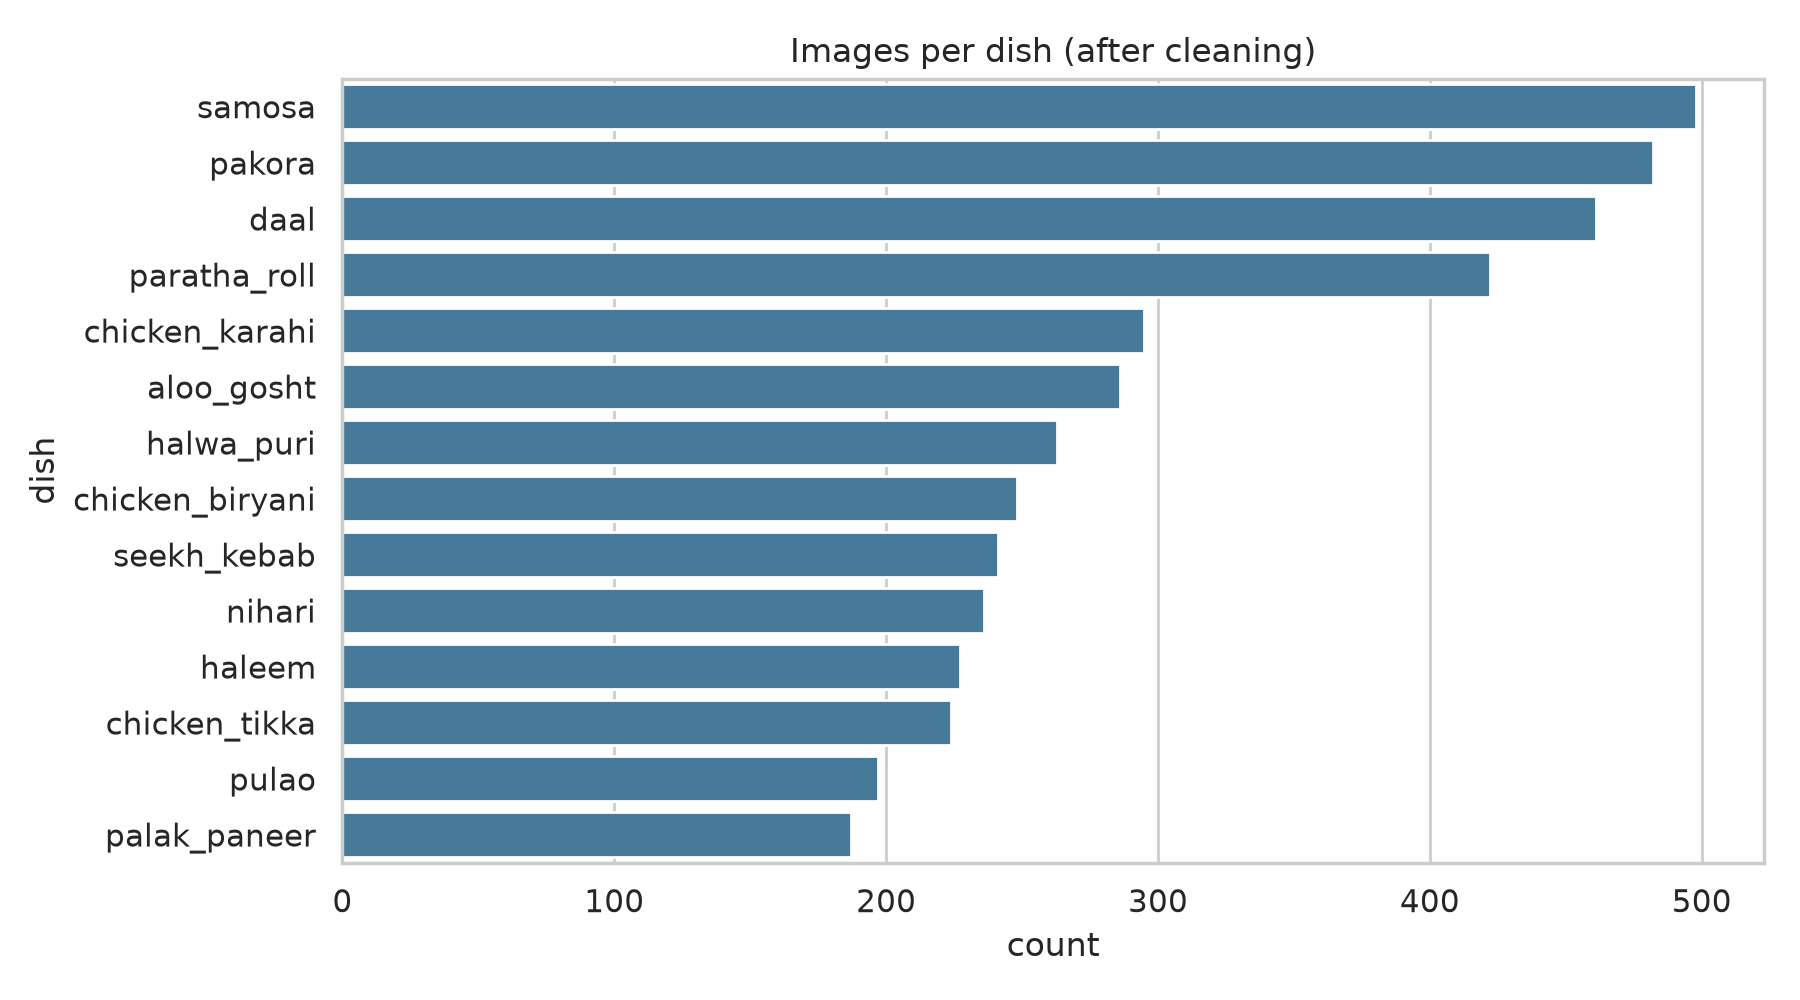
\includegraphics[width=0.85\textwidth]{class_distribution.png}
  \caption{Images per dish after cleaning.}
\end{figure}
The classes are imbalanced. Samosa has the most images (498) and palak\_paneer the fewest (187), a ratio of about 2.7 to 1. The four largest classes (samosa, pakora, daal and paratha\_roll) are exactly the four dishes that also draw on the Kaggle dataset.

\begin{figure}[H]
  \centering
  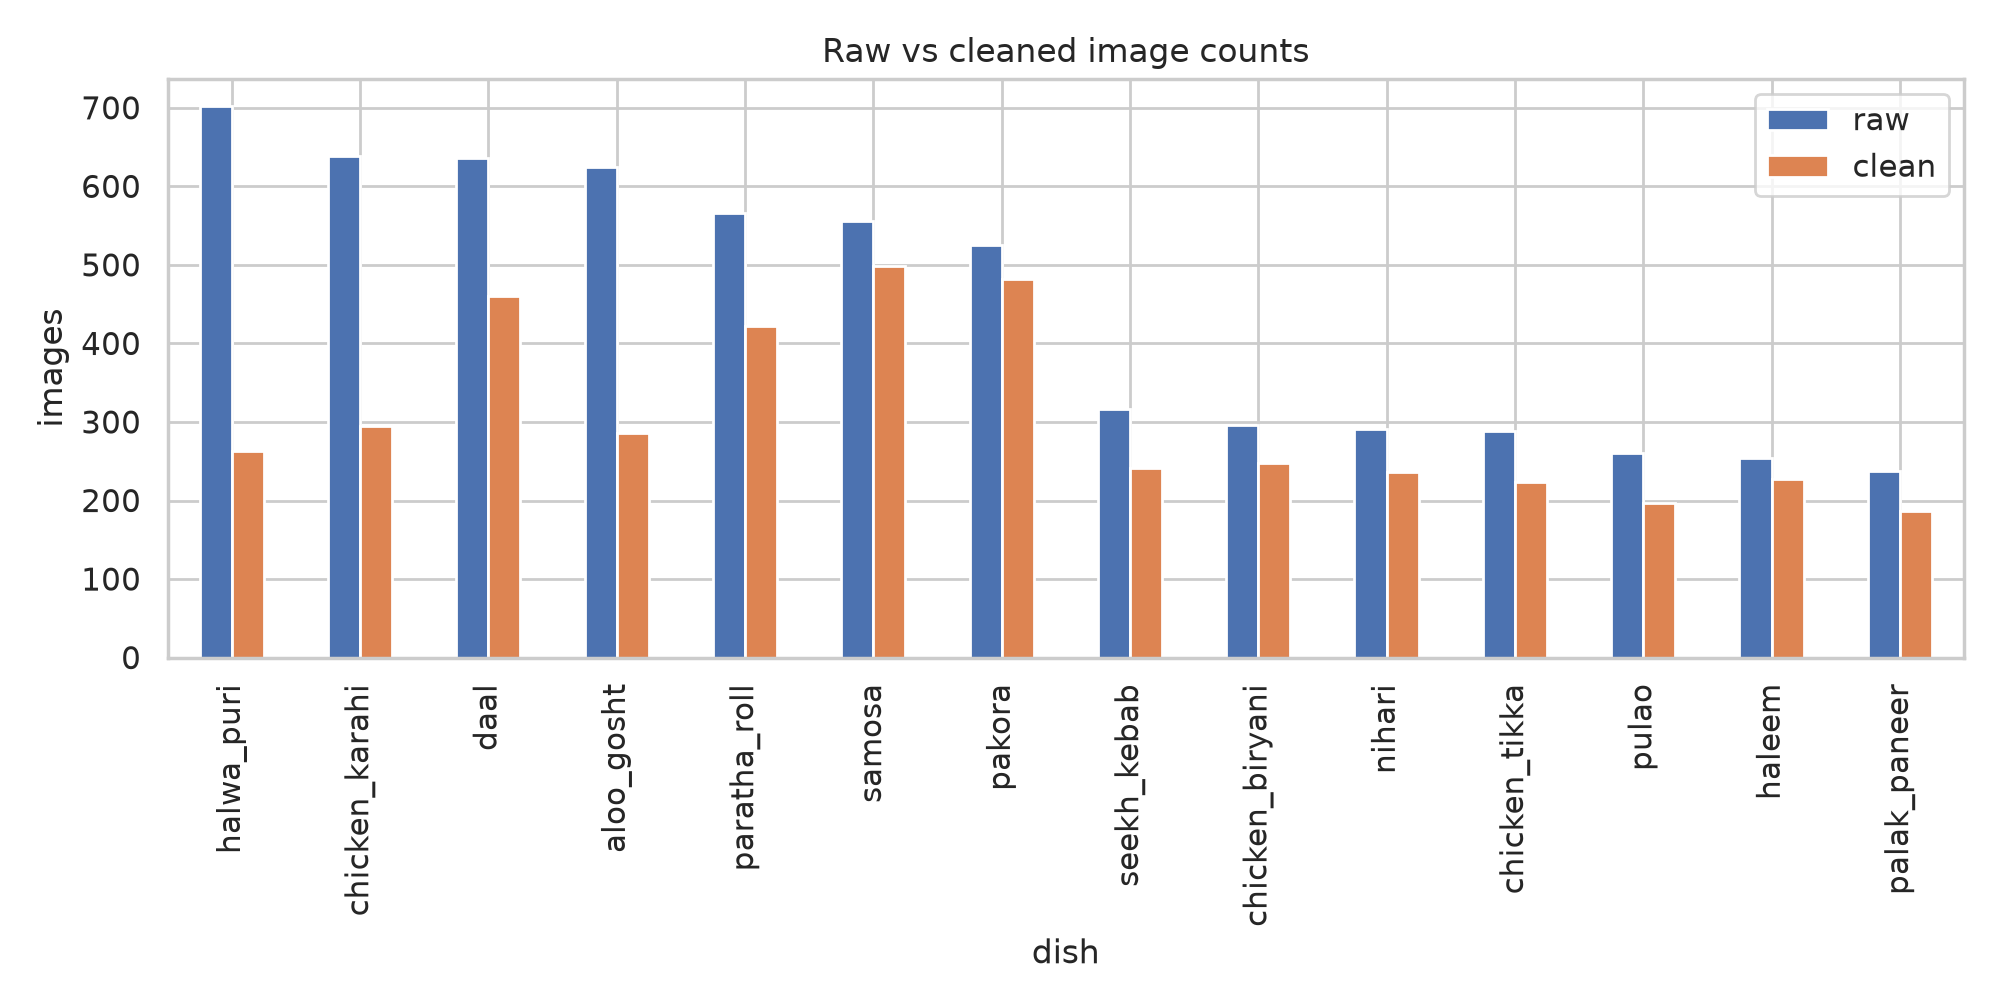
\includegraphics[width=0.85\textwidth]{raw_vs_clean.png}
  \caption{Raw versus cleaned image counts.}
\end{figure}
Cleaning reduced the collection from 6,193 to 4,267 images, and every dish lost some images. The largest shares were lost by halwa\_puri (439 of 702, about 63\%), aloo\_gosht (338 of 624, about 54\%) and chicken\_karahi (344 of 639, about 54\%), which are the three dishes that received top-up scraping and therefore contained many repeated downloads. Pakora lost the smallest share (43 of 525, about 8\%).

\begin{figure}[H]
  \centering
  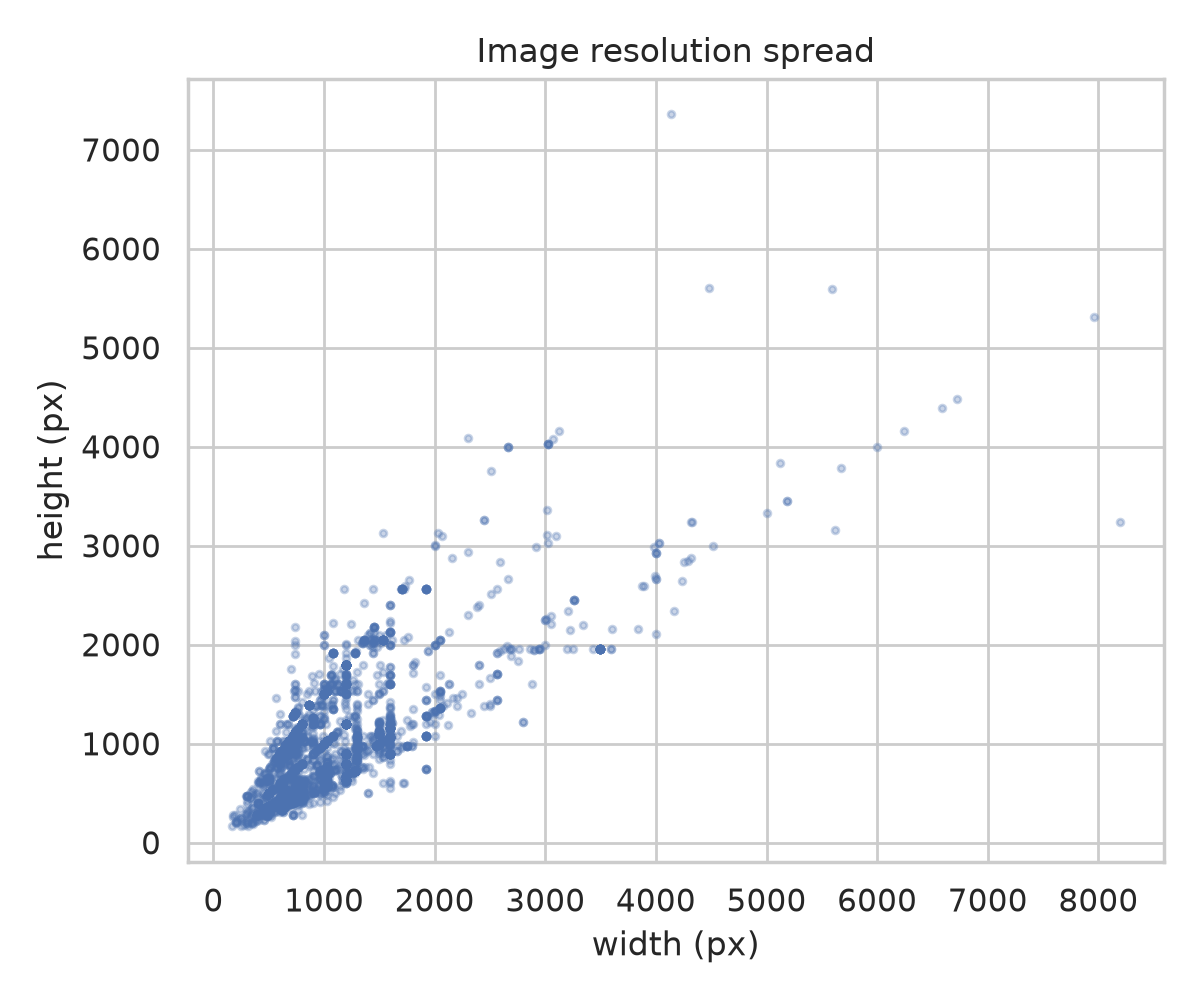
\includegraphics[width=0.6\textwidth]{image_sizes.png}
  \caption{Image resolution spread.}
\end{figure}
Image resolution varies widely, from small images of a few hundred pixels to a few very large ones more than 4,000 pixels wide, and width and height grow together. This spread motivates resizing everything to a common $224 \times 224$ input.
% TODO: add the typical range (for example "most images are below about N pixels") after checking the new image_sizes.png.

\begin{figure}[H]
  \centering
  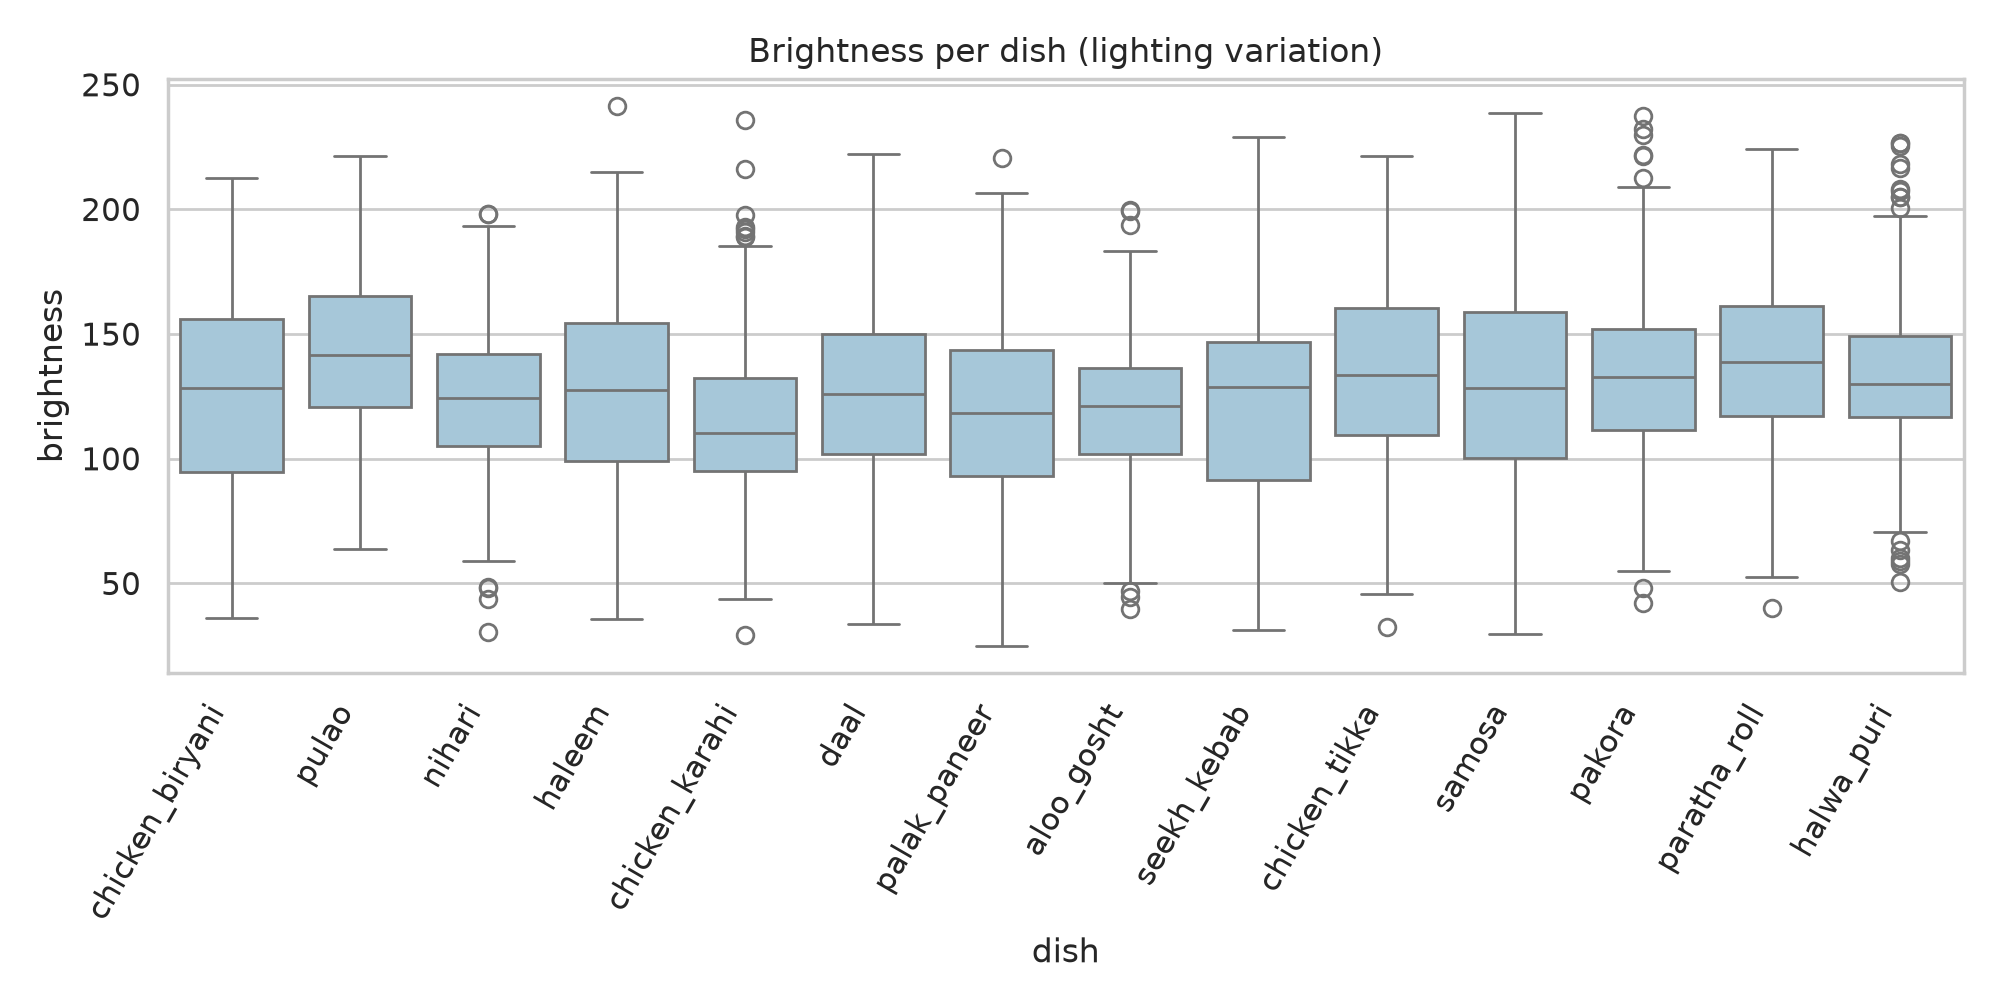
\includegraphics[width=0.85\textwidth]{brightness_per_dish.png}
  \caption{Brightness per dish (lighting variation).}
\end{figure}
Brightness varies widely within every dish, so each dish contains both dark and bright photos, and lighting differs between individual images more than it differs between dishes.
% TODO: add the median range per dish (darkest and brightest dish) after checking the new brightness_per_dish.png.

\begin{figure}[H]
  \centering
  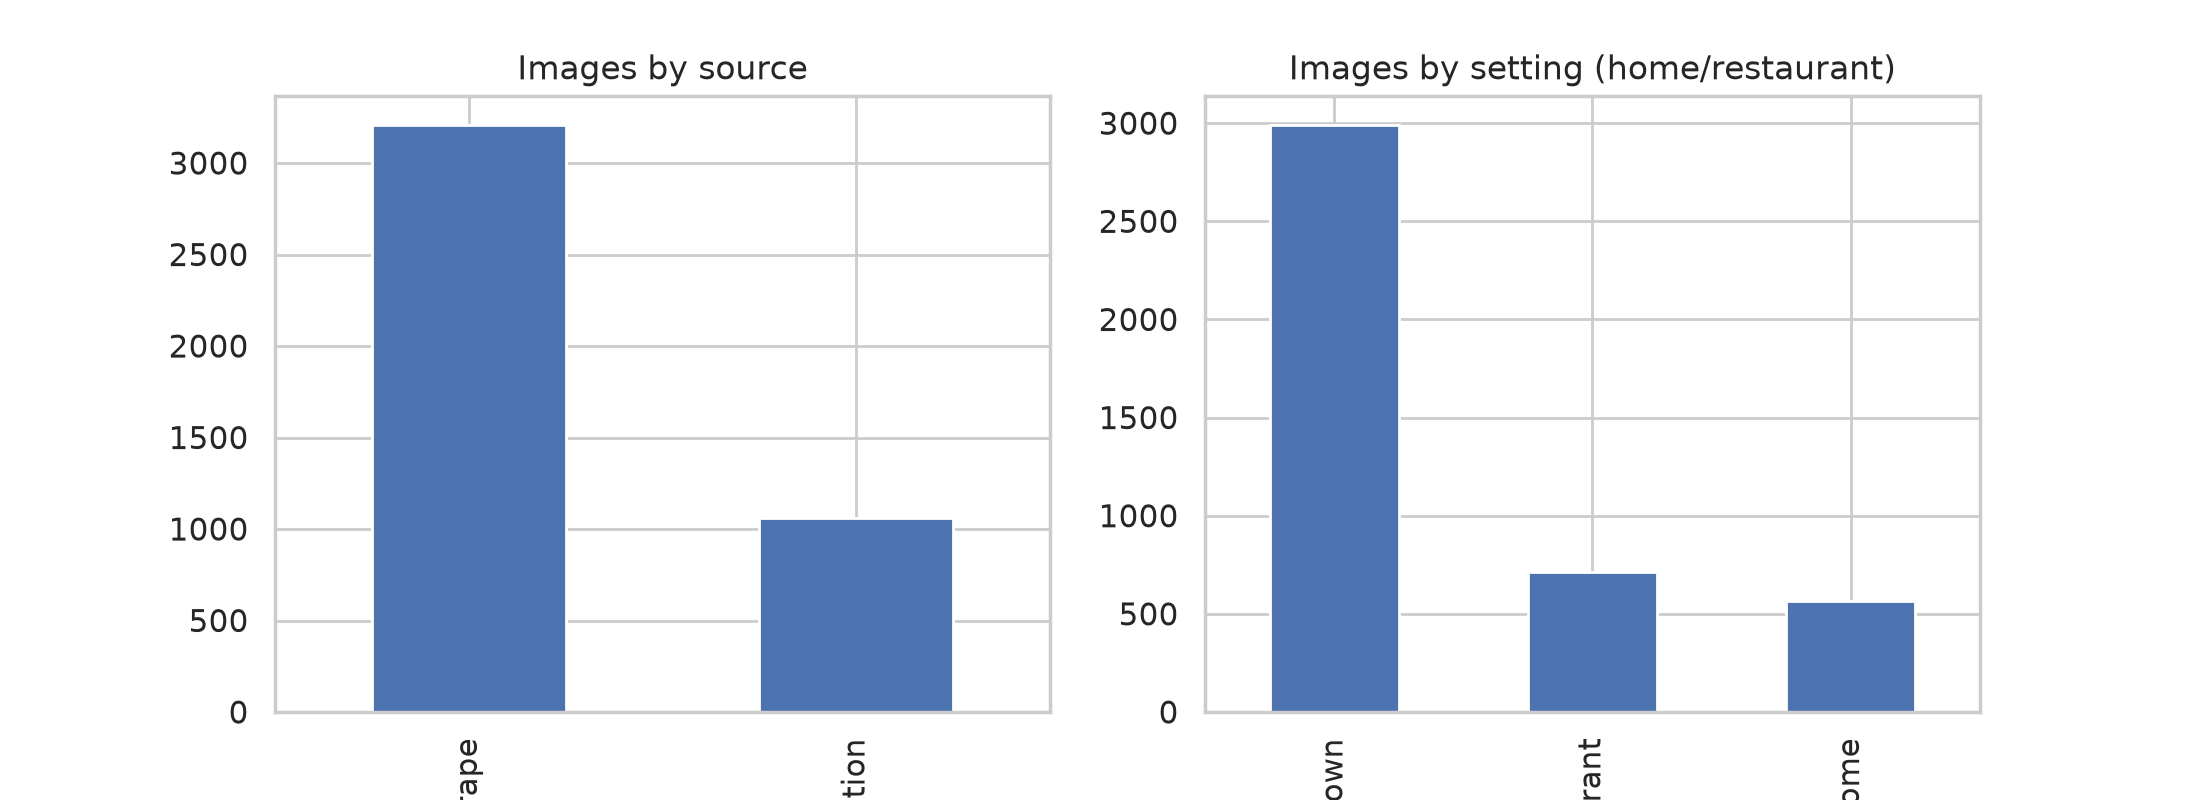
\includegraphics[width=0.85\textwidth]{source_and_setting.png}
  \caption{Images by source and by setting (home/restaurant).}
\end{figure}
Most of the cleaned images come from Bing, and a smaller share from the Kaggle dataset. The setting is unknown for most images, because only some of the search queries mention a home or restaurant setting and the Kaggle images carry no setting label.
% TODO: add the exact Bing/Kaggle percentages and the home/restaurant/unknown split after checking the new source_and_setting.png.

\begin{figure}[H]
  \centering
  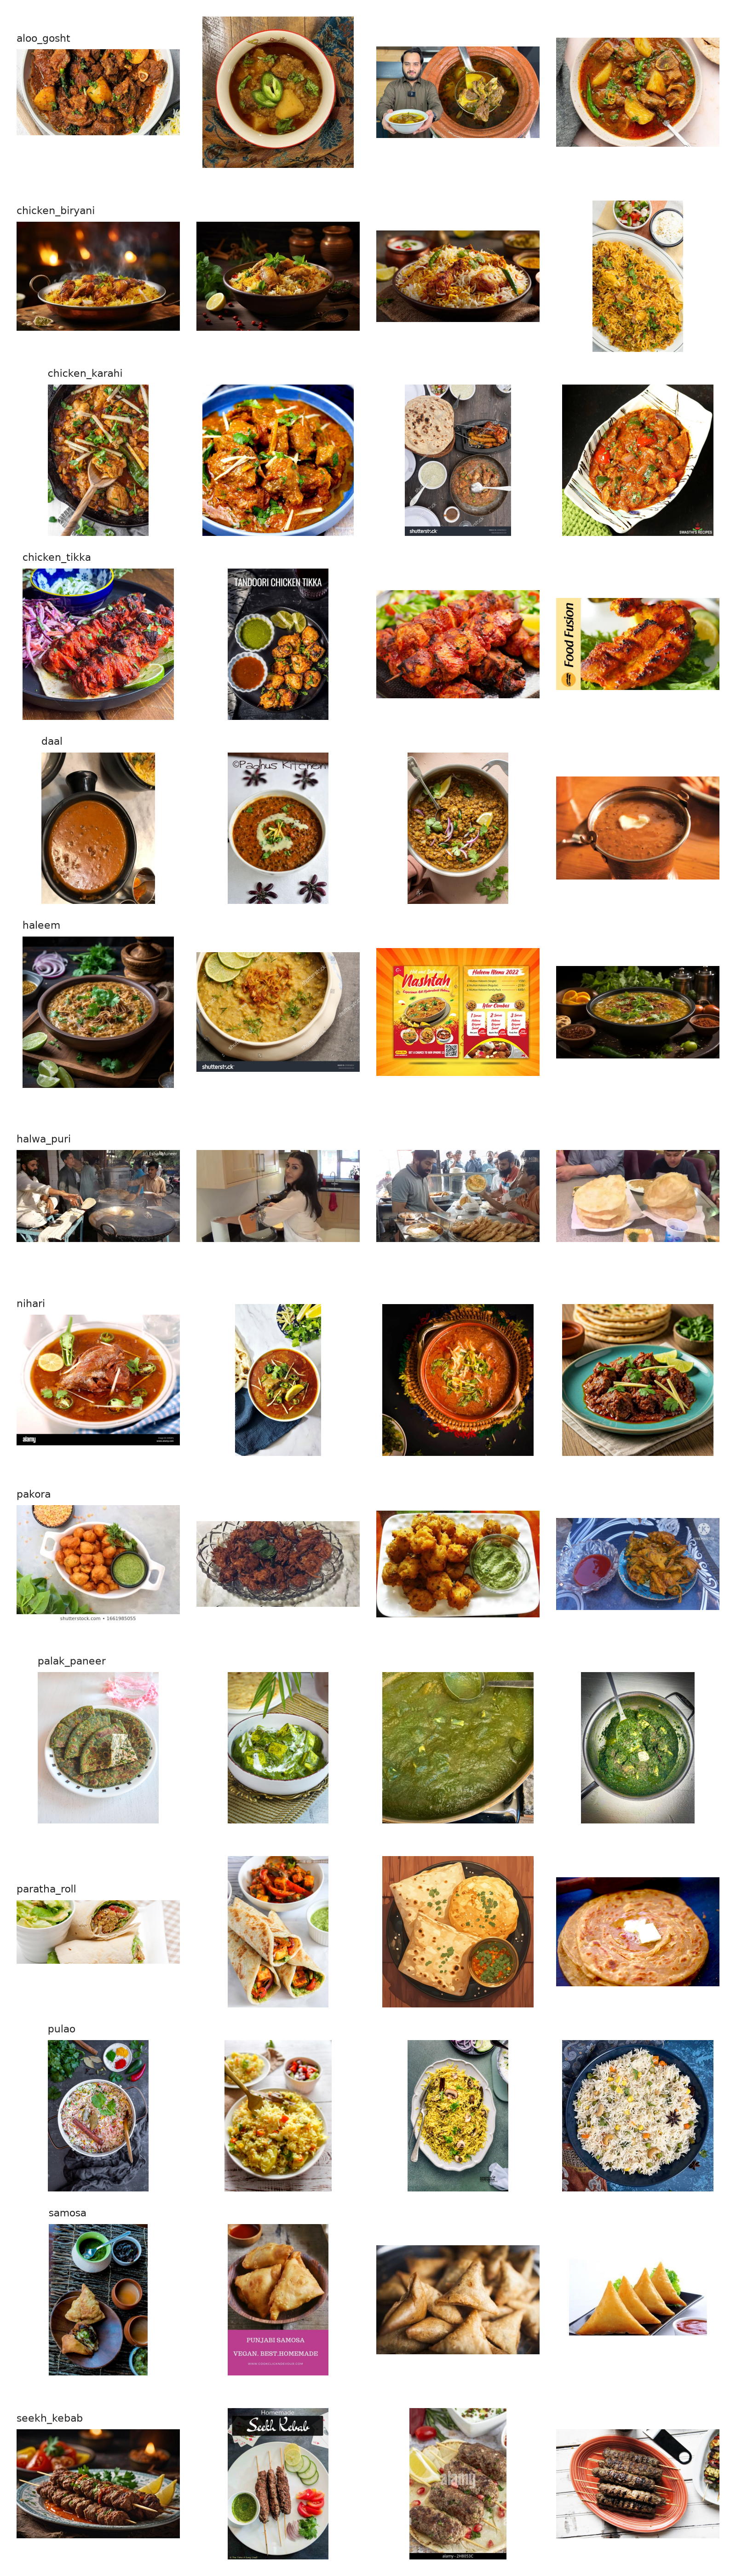
\includegraphics[width=0.7\textwidth]{sample_grid.png}
  \caption{Random samples per dish.}
\end{figure}
The sample grid shows four random cleaned images per dish. The images vary widely in angle, plating and background. The grid also exposes the problems listed under the limitations, such as watermarks, text overlays and occasional images that do not show the labelled dish.
% TODO: re-check against the new sample_grid.png and mention specific examples if they appear.

\subsection{Limitations}
\begin{itemize}
  \item \textbf{Watermarks and text overlays:} images scraped from Bing can contain watermarks, captions or text overlays, which the automatic blur and duplicate filters do not remove. Stock-photo watermarks (for example Alamy and Shutterstock), text banners (many in Urdu), video-thumbnail graphics with a ``subscribe'' button or a presenter's face, and even a menu page were found in the cleaned images. In a random sample of 24 images per dish, about half of the aloo\_gosht and halwa\_puri images (the dishes with the most top-up images) and about one in five chicken\_karahi images were affected. Some banners even repeat the dish name, so a model could learn to read the text instead of recognising the food.
  \item \textbf{Label noise:} a few cleaned images do not appear to show the labelled dish or are not photographs of food (for example a cartoon illustration and a plate of chaat among the halwa\_puri images, a restaurant menu page among the chicken\_karahi images, and off-topic images in palak\_paneer). The cleaning filters cannot detect these and the dataset was reviewed only by sampling, so some mislabelled images probably remain.
  \item \textbf{Source bias:} four dishes (samosa, pakora, daal and paratha\_roll) draw on a single Kaggle dataset, while the other ten come only from Bing. The two sources may differ in photographic style, so a model could partly learn the source instead of the dish.
  \item \textbf{Close substitutes:} the Kaggle classes \texttt{dal\_makhani} and \texttt{kaathi\_rolls} stand in for daal and paratha\_roll. They are similar dishes but not identical to what the project is meant to recognise.
  \item \textbf{Class imbalance:} raw counts range from 237 to 702 images per dish and cleaned counts from 187 to 498. All 14 dishes are above our 150-image target, but only after the top-up scraping (chicken\_karahi was at 128 after the first cleaning). The smallest class, palak\_paneer, has 187 images, so with a 15\% split its validation and test sets hold only about 28 images each and its per-class results will be noisy.
  \item \textbf{Repeated downloads:} the top-up queries returned many images that were already collected, so a large part of the new downloads was removed as duplicates. The three top-up dishes therefore keep a smaller share of their raw images than the others. Some near-duplicates still survive: in the aloo\_gosht sample, what appears to be the same photo occurs twice with different crops, which the perceptual-hash threshold did not catch.
  \item \textbf{Licensing:} the scraped images belong to their original owners. They were collected for academic use only and are not redistributed: the dataset is excluded from the repository.
\end{itemize}
